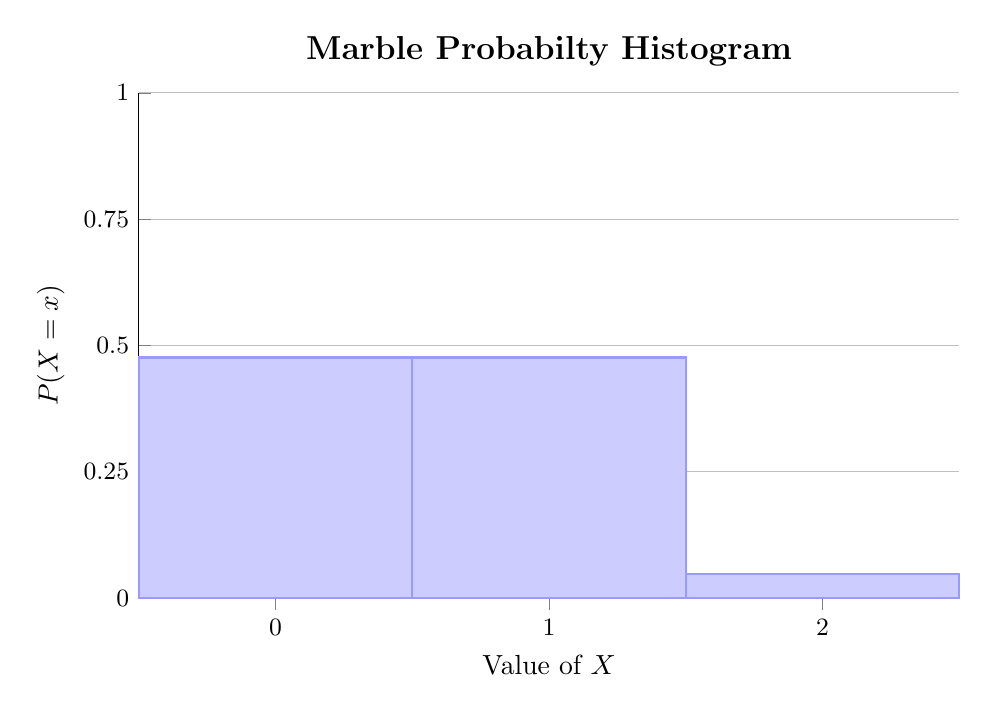
\begin{tikzpicture}
  \begin{axis}[
      axis lines*=left,
      no markers,
      xmin=-0.5, xmax=2.5, ymin=0, ymax=1,
      xtick={0,1,2},
      ytick={0,0.25,0.5,0.75,1},
      xlabel={Value of $X$},
      ylabel={$P(X=x)$},
      title={\large\bf Marble Probabilty Histogram},
      ticklabel style={font=\small},
      enlargelimits=false,
      clip=false,
      grid = none,
      ymajorgrids=true,
      ybar=0pt,
      bar width=1,
      width=12cm,
      height=8cm
    ]
    \addplot+[thick,fill=blue!20,draw=blue!40] coordinates { 
        (0, 0.4762)
        (1, 0.4762)
        (2, 0.0476)
    };
  \end{axis}
\end{tikzpicture}
